\documentclass[a4paper,12pt]{article}
\usepackage{graphicx}
\usepackage{verbatimbox}
\usepackage{caption}
\usepackage{here}
\usepackage{amsmath}
\usepackage{fancyvrb}
\usepackage{lipsum}
\usepackage{hyperref}
\begin{document}

\title{UROP Report}
\author{Francesco Barbara, Tin-Yu Hui}
\maketitle
\pagenumbering{arabic}
\section{Modelling assumptions}
All the analyses present in this report are carried out on \textbf{pairs of biallelic non-coding loci}.
This means that if you have a $m\cdot n$ haplotype matrix (where $m$ is the number of gametes and $n$ is the number of loci), you can carry out $n^2$ independent analyses.\\

The model used throughout the UROP was a standard Wright-Fisher model (WF). WF describes a population with discrete, nonoverlapping generations. In each generation the entire population is replaced by the offspring from the previous generation.
Each new gamete, is sampled with replacement from the parent generation gamete pool. Recombination happens with probability c.
The WF model includes evolutionary forces such as recombination,
 genetic drift (i.e. variability due to random sampling of gametes)
 and migration (when multiple populations are taken into consideration), but fails to take into account other forces such as mutation
and selection (which in this case is unnecessary as we work with non-coding loci).




\section[Section Title. Section Subtitle]{Single population linkage disequilibrium r\textsuperscript{2} measure\\ {\small Common population based simulators, and recursive deterministic approaches both fail to describe the true trajectory of $r^{2}$ over time}}
Simulating a full population of diploid individuals throughout time is computationally demanding. For example, simulating a small population of size 1000, for 100 generations, already requires 200,000 gametes to be simulated.\\

A commonly used shortcut  for approximating the behaviour of the $r^2$ is to use a  \textbf{population-based simulator}.
Rather than simulating all individuals, it only keeps track of the 4 joint haplotype frequencies $\{p_1, p_2, p_3,p_4 \}$  and updates them at each generation.
This approach treats the recombination effect deterministically (by making a fixed adjustment to the frequencies depending on the recombination rate and the current raw LD measure), and the random mating effect stochastically (using multinomial sampling with size $2N_e$, i.e. twice the population size).\\

A second fully determistic approach, is using the following \textbf{recursion}:\\
$$ E(r^2_{t+1}) \approx \frac{1}{2N_e} + (1 -  \frac{1}{2N_e}) (1- c^2) r^2_{t} $$
In addition, beacuse there is no randomness involved, this approach does not allow us to find confidence intervals if for example we want to infer the population size (put it in simple terms, we don’t know how “noisy” the observations are).\\

Park (2012) proposes an updated recursion which deals quite well with the single population case. However, cannot be extended if we want to take migration into account, plus the same remark on confidence intervals still applies in this case.\\
$$ E(r^2_{t+1}) \approx \frac{1}{2N_t} + \frac{c^2}{2N_{t-1}} + (1 - \frac{c}{N_{t-1}})(1 -  \frac{1}{2N_t}) (1- c^2) r^2_{t} $$ \\

With the aim of comparing these 3 approaches with the individual based simulator (which describes WF exactly), I ran 10,000 simulations and took the average $r^2$ for each generation, under different scenarios. The results showed that for small recombination rates, the population based simulator and the basic recursion were almost unbiased, while for higher recombination rates, they had a significant downward bias. Park's recursion, on the other hand, perfomed well in  the different scenarios.\\

The scenarios tested were:\\

 $N_e = 1000$ for generations 1 to 50; recombination rate in $\{0.01, 0.1, 0.2, 0.3, 0.4, 0.5\}$\\
 
 $N_e = 1000$ for generations 1 to 25, $N_e = 5000$ for generations 26 to 50; recombination rate in $\{0.01, 0.1, 0.2, 0.3, 0.4, 0.5\}$\\
 
All the code and plots are available at:\\
\url{https://github.com/francescobarbara/UROP/tree/main/Park%20(2012)}

\begin{figure}[H]
    \centering
    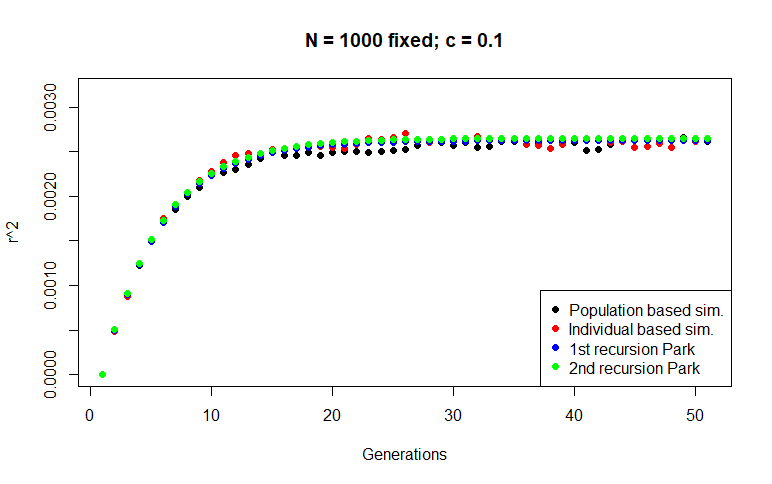
\includegraphics[scale=0.7]{1.png}%
    \caption*{Figure (1): Average $r^2$ over 10,000 simulations; $N_e = 1000$, recombination rate $= 0.1$}% 
\end{figure}%

\begin{figure}[H]
    \centering
    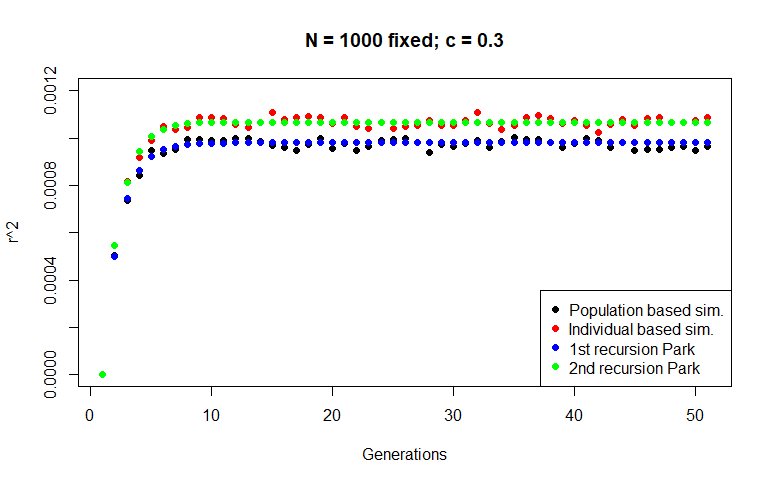
\includegraphics[scale=0.7]{2.png}%
    \caption*{Figure (2): Average $r^2$ over 10,000 simulations; $N_e = 1000$, recombination rate $= 0.3$}% 
\end{figure}%

\begin{figure}[H]
    \centering
    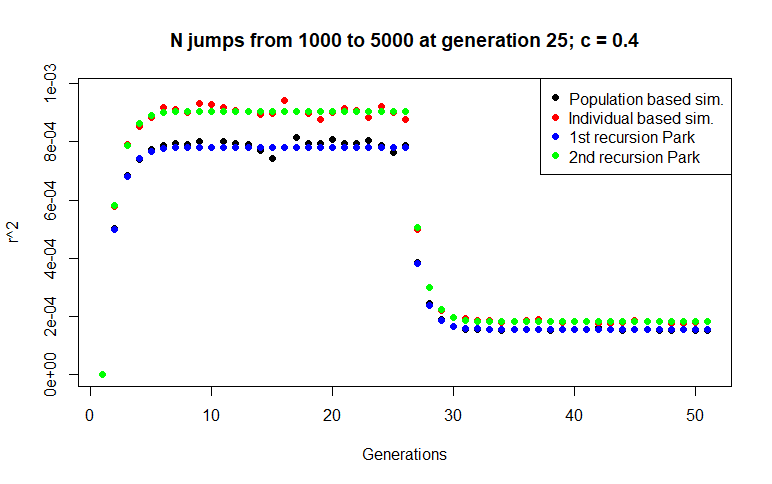
\includegraphics[scale=0.7]{3.png}%
    \caption*{Figure (3): Average $r^2$ over 10,000 simulations; $N_e$ jumps from 1000 to 5000, recombination rate $= 0.4$}% 
\end{figure}%
\pagebreak

\section{Two-populations individual-based simulator}
The above investigation highlighted how neither multinomial sampling (two multinomial samplings per generation of sizes $N_e$ or $2N_e$ were also tried, giving unsatisfying results) nor the commonly used recursion manage to approximate suffieciently well the motion of the $r^2$ under the WF model. The recursion in Park (2012) is only a partial solution, as it only deals with isolated populations, and it fails to give an idea on the variance of $r^2$, making parameters inference infeasible.\\

This emphasised the need for the development of an efficient individual-based simulator. The underlying model is straightforward.\\
There are two populations (whose sizes throughout the generations $N_t$ and $M_t$ can vary) and fixed migration rates (for example, $m_{12} = 0.15$ means that at each generation 15\% of the individuals in population 1 will migrate to population 2).\\
At each generation, we initially have a migration phase, where individuals are sampled and moved from on population to the other, then we have a reproduction phase, where each population reproduces independently according to the WF model.

\begin{figure}[H]
    \centering
    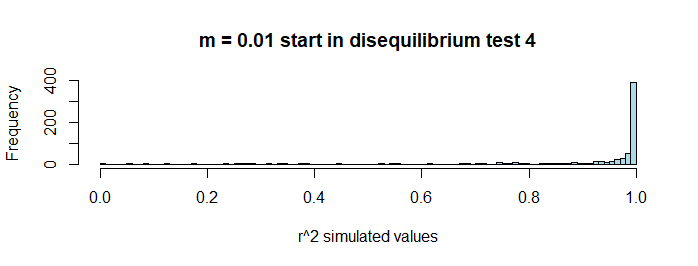
\includegraphics[scale=0.8]{4.png}%
    \caption*{Figure (4): Model for two migrating populations}% 
\end{figure}%
\pagebreak

The core functions were written in the programming language C++. Nevertheless, it is very easy to run the simulator within an R console by installing the package $Rcpp$  (which works as a bridge between R and C++).\\
100 generations for populations sizes $N_e, M_e < 100,000$ are simulated in less than a second on a standard laptop; for $N_e, M_e = 1,000,000$ it takes around 15 seconds.\\

All the code and instructions are available at:\\
\url{https://github.com/francescobarbara/UROP/tree/main/C%2B%2B_code_for%20_two_pop}

\section{Population size estimation using  r\textsuperscript{2}}
Suppose we want to estimate $N_e$ (we assume fixed populations size), the best tool we have at our disposal so far, is the recursion introduced by Park (2012). We can invert the relationship below and get an estimate for the population size.
$$ E(r^2_{t+1}) \approx \frac{1}{2N_t} + \frac{c^2}{2N_{t-1}} + (1 - \frac{c}{N_{t-1}})(1 -  \frac{1}{2N_t}) (1- c^2) r^2_{t} $$ \\
Having a migration flux, makes our estimates perform poorly and leads to a significant upward bias (i.e. $N_{e}^{est}  >> N_e $ )\\
In tables (5) and (6), I do 10,000 simulations for each migration-recombination rate pair, take the average of the 10,000 estimated population sizes and return the ratio between the population estimate and the true population size.
It can be seen that the upward bias increases as migration grows and the recombination rate decreases.

\begin{figure}[H]
    
    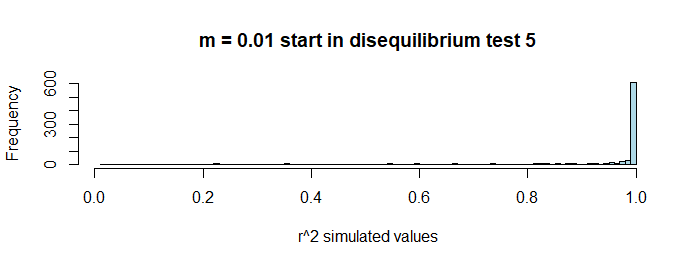
\includegraphics[scale=0.9]{5.png}%
    \caption*{Table (5): $N_e = 1000$, $M_e = 1000$, for each (c, migration) pair $N_{e}^{est} / N_e $  is returned}% 
\end{figure}%

\begin{figure}[H]
    
    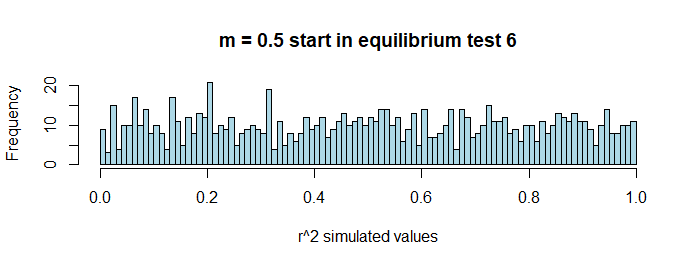
\includegraphics[scale=0.85]{6.png}%
    \caption*{Table (6): $N_e = 1000$, $M_e = 10,000$, for each (c, migration) pair $N_{e}^{est} / N_e $ is returned}% 
\end{figure}%

\section{Between population LD measure}
From the previous section, it is clear that, despite the fact that $r^2$ gives unbiased estimates for the size of a single isolated population, when migration comes into play the results are not satisfying.\\
Similarly to the way $r^2$ measures \textbf{within population} linkage disequilibrium, the need for developing a measure of  \textbf{between population} linkage disequilibrium arised.\\

Suppose you have two 2x2 contingency tables (one for each of the two populations) containing the 4 joint haplotype frequencies.
You can create a \textbf{2x2x2 contingency table} by putting all the observations together and using as `third axis' of the table, the population to which each observation belongs.\\
More formally, let  $2N_e$ and $2M_e$ be the sample sizes for population 0 an population 1 (we are working under the assumption of exhaustive sampling, but the measure generalises). Then $O_{011} = q_2*\frac{2M_e}{2N_e + 2M_e}$; that is  $O_{011}$ is the number of gametes that have gene 0 at the first locus, gene 1 at the second locus and are in population 1, divided by the total number of gametes in the two populations.

\begin{figure}[H]
    
    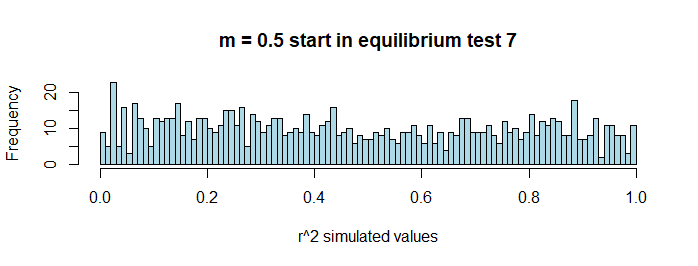
\includegraphics[scale=0.8]{7.png}%
    \caption*{Figure (7): Creation of the 2x2x2 contingency table}% 
\end{figure}%

The measure developed (which we call $l^2$) is the p-value of a likelihood ratio test.
The \textbf{null} hypotesis of the test is that the 2 samples come from the same population, and the population is in equilibirium.
The \textbf{alternative} hypotesis is that the 2 populations are independent (i.e. the migration rate
between the two is zero) and each population is in equilibrium when considered singularly.\\

\noindent $H_0: \quad O_{ijk} = \alpha_{i}\cdot\beta_{j}\cdot\gamma_{k} \qquad \forall \:(i,j,k)\; in\; \{0,1\}^3$ \\

 $ \qquad s.t. \quad \alpha_{0} +\alpha_{1} = 1; \: \beta_{0} + \beta_{1} = 1; \: \gamma_{0} + \gamma_{1} = 1; \: O_{000}
 +...+O_{111}=1    $\\
 
 $ \implies dim(H_{0}) = 3 $\\
 
 \noindent $\alpha_{0}$ and $\alpha_{1}$ are the marginal frequencies of alleles `0' and `1' respectively at Locus 1.\\
 \noindent $\beta_{0}$ and $\beta_{1}$ are the marginal frequencies of alleles `0' and `1' respectively at Locus 2.\\
 \noindent  $\gamma_{0}$ and $\gamma_{1}$ represent the frequencies of population 0 and population 1 over the whole set; i.e.
 $\gamma_{0} = N_e / (N_e + M_e) \: ; \: \gamma_{1} = M_e / (N_e + M_e)$  \\
 
 \noindent $H_1: \quad O_{ij0} = \alpha_{i}\cdot\beta_{j}\cdot\epsilon_{0} \quad O_{ij1} = \gamma_{i}\cdot\delta_{j}\cdot\epsilon_{1}$\\
 
 $ \qquad s.t.  \quad \alpha_{0} +\alpha_{1} = 1; \: \beta_{0} + \beta_{1} = 1; \: ... \:; \epsilon_{0} + \epsilon_{1} = 1; \; O_{000}+...+O_{111}=1    $\\
 
  $ \implies dim(H_{1}) = 5 $\\

 \noindent $\alpha_{0}$ and $\alpha_{1}$ are the marginal frequencies of alleles `0' and `1' respectively at Locus 1 for population 0.\\
 \noindent $\beta_{0}$ and $\beta_{1}$ are the marginal frequencies of alleles `0' and `1' respectively at Locus 2 for population 1.\\
  \noindent $\gamma_{0}$ and $\gamma_{1}$ are the marginal frequencies of alleles `0' and `1' respectively at Locus 1 for population 1.\\
 \noindent $\delta_{0}$ and $\delta_{1}$ are the marginal frequencies of alleles `0' and `1' respectively at Locus 2 for population 1.\\
 \noindent  $\epsilon_{0}$ and $\epsilon_{1}$ represent the frequencies of population 0 and population 1 over the whole set.\\
 
 \noindent Essentially in $H_{1}$ each population has its own $\alpha$ and $\beta$, because the two populations are disjoint.\\
 
 A common test, when $H_0$ and $H_1$ have nested parameter spaces, is the likelihood ratio test (LRT). It assumes that the following test statistic is distributed according to a chi squared random variable with degrees of freedom equal to $dim(H_1) - dim(H_0)$:
 $$\Lambda = 2(sup_{H_1}(l(\pi)) - sup_{H_0}(l(\pi)) ) \approx \chi^2_{5-3} = \chi^2_{2}  $$
 Remark: $sup_{H_1}(l(\pi))$ means the maximum log-likelihood taken over all possible parameters satisfying $H_1$.\\
 
Let $n_{ijk}$ be the count of gametes in cell $(i,j,k)$ of the 2x2x2 contingency table (assuming we have $2N_e + 2M_e$ total gametes, then $O_{ijk} = n_{ijk}/(2N_e + 2M_e)$).\\
Let's use notation $n_{\bullet j \bullet}$ to indicate all the marginal counts.\\
For example, \\
\noindent we use   $n_{0 \bullet  \bullet}$ to indicate the number of gametes that have gene 0 at the first locus;\\
\noindent we use   $n_{\bullet 1 \bullet}$ to indicate the number of gametes that have gene 1 at the second locus;\\
\noindent we use  $n_{\bullet  \bullet 0}$ to indicate the number of gametes that are in population 0.\\
 
 Then, under $H_0$, if we assume a multinomial model, the maximum likelihood estimates $\hat{\alpha}$, $\hat{\beta}$, $\hat{\gamma}$, will be the marginal frequencies. \\
 \noindent That is $\hat{\alpha_0} = n_{0 \bullet  \bullet}/(2N_e + 2M_e), \:... \:, \: 
\hat{\gamma_1} = n_{ \bullet  \bullet 1}/(2N_e + 2M_e) $\\

\noindent Therefore the maximum likelihood under $H_0$ is, using multinomial distribution of the gametes:\\
$$sup_{H_0}(L(\pi)) = \sum_{i = 0}^1  \sum_{j = 0}^1  \sum_{k = 0}^1 {2N_e + 2M_e \choose n_{ijk}} (\hat{\alpha} \cdot \hat{\beta} \cdot \hat{\gamma})^{n_{ijk}} = $$
 $$\sum_{i = 0}^1  \sum_{j = 0}^1  \sum_{k = 0}^1 {2N_e + 2M_e \choose n_{ijk}}(\frac{n_{i \bullet  \bullet}
 n_{ \bullet j \bullet}n_{\bullet  \bullet k}}{(2N_e + 2M_e)^3}) ^ {n_{ijk}}$$
 For simplicity, let's call the quantity in the parenthesis $E_{ijk}$ (the expected frequency of cell (i,j,k) under the null).\\
 By taking the logarithm of the above expression, we get that the log likelihood is:
 $$sup_{H_0}(l(\pi)) = \sum_{i = 0}^1  \sum_{j = 0}^1  \sum_{k = 0}^1 n_{ijk}\cdot log(E_{ijk}) \quad + \quad const$$
 Remark: the constant term will cancel out with the constant term of $sup_{H_1}(l(\pi))$\\
 
\noindent Similarly, under $H_1$, we can approximate expected frequency of each cell (i,j,k) with the observed frequency $O_{ijk}$.\\ 

\noindent Remark: This is not formally 100\% correct. In theory we would have to pick parameters $\alpha$, $\beta$, $\gamma$, $\delta$, $\epsilon$ such that they maximise the likelihood. In practice, becuase the observed data satisfies the physical assumptions of $H_1$, the difference would be minimal. Therefore I opted for a more interpretable formula, which uses directly the observed frequencies $O_{ijk}$ (rather than some numbers that are essentially the observed frequencies with some very small noise)  
  $$sup_{H_1}(l(\pi)) = \sum_{i = 0}^1  \sum_{j = 0}^1  \sum_{k = 0}^1 n_{ijk}\cdot log(O_{ijk}) \quad + \quad const$$ 
   $$\Lambda = 2(sup_{H_1}(l(\pi)) - sup_{H_0}(l(\pi)) ) = 2 \cdot \sum_{i = 0}^1  \sum_{j = 0}^1  \sum_{k = 0}^1 n_{ijk}\cdot log(O_{ijk}/E_{ijk}) $$
   
\noindent Now, $O_{ijk}$ and $E_{ijk}$ are frequencies, while $n_{ijk}$ is a count (so grows lineraly with respect to the total number of gametes). Thinking about scenarios in which exhaustive sampling is not possible, I thought that a linear dependence with respect to the sample size, was not ideal, hence I decided to change $n_{ijk}$ into $O_{ijk}$
  
  $$\Lambda = 2 \cdot \sum_{i = 0}^1  \sum_{j = 0}^1  \sum_{k = 0}^1 O_{ijk}\cdot log(O_{ijk}/E_{ijk}) $$
  
\noindent This essentially changes the `scale' we are working on by an approximate factor of $1/(2N_e + 2M_e)$. You must think that now the assumption $\Lambda \approx  \chi^2_{2} $ does not hold anymore. This was however a very arbitrary assumption (it was not at all based on physical considerations), we simply wanted some random variable taking values in $[0, \infty)$ that would allow us to differentiate migration rates. Therefore I opted for the final formula, which does not over-react to non-exhaustive sampling and in the following section was shown to differentiate migration rates quite well.

$$ l^2 := Prob(\chi_2^2 \le \Lambda_{observed})$$

\subsection {A worked example}
For explanatory purposes, let's go through an example.\\
\noindent Let $p = \{0.25, 0.25, 0.25, 0.25\}$, $N_e = 1000$, $q = \{0.32, 0.25, 0.25, 0.18\}$, $M_e = 4000$.
Then the matrix of observed frequencies $O$ is (showing the two 2x2 layers separately):
$$ O =
\begin{bmatrix}
0.05 & 0.05\\
0.05 & 0.05
\end{bmatrix} 
\begin{bmatrix}
0.256 & 0.2\\
0.2 & 0.144
\end{bmatrix} 
$$
\noindent Calculating the marginals:\\

\noindent $\hat{\alpha_{0}} = 0.05+0.05+0.256+0.2 = 0.556$\\
\noindent $\hat{\alpha_{1}} = 0.05+0.05+0.2+0.144 = 0.444$\\
\noindent $\hat{\beta_{0}} = 0.05+0.05+0.256+0.2 = 0.556$\\
\noindent $\hat{\beta_{1}} = 0.05+0.05+0.2+0.144 = 0.444$\\
\noindent $\hat{\gamma_{0}} = 0.05+0.05+0.05+0.05 = 0.2$\\
\noindent $\hat{\gamma_{1}} = 0.256+0.2+0.2+0.144 = 0.8$\\

\noindent Creating the matrix of expected frequencies under the null $E$, where $E_{ijk} = \alpha_i \beta_j \gamma_k$
$$ E =
\begin{bmatrix}
0.0618 & 0.494\\
0.0494 & 0.394
\end{bmatrix} 
\begin{bmatrix}
0.247 & 0.197\\
0.197 & 0.158
\end{bmatrix} 
$$
  $$\Lambda_{observed} = 2 \cdot \sum_{i = 0}^1  \sum_{j = 0}^1  \sum_{k = 0}^1 O_{ijk}\cdot log(O_{ijk}/E_{ijk}) = 0.00664$$
$$ l^2 := Prob(\chi_2^2 \le \Lambda_{observed}) = 0.0033$$  

\subsection {Does l\textsuperscript{2} manage to catch migration signals?}
To this purpose, I test several cases with different migration rates, while all of the other parameters are kept fixed.
The other parameters are: $N_e = 1000$, $M_e = 1000$, $generations = 100$, $c = 0.1$, initial frequencies are in equilibrium $p_0, q_0 = \{0.25,0.25,0.25,0.25\}$.\\
\noindent Migration rates are $\{0.001, 0.05, 0.1, 0.2, 0.3, 0.4, 0.5\}$.\\

\noindent For each of these rates I do 1000 simulations. For each simulation I simulate the 100 generations using the C++ script, then I consider the frequencies p and q at generation 100, and make a LR test on these final frequencies. I store all the 1000 $l^2$ values (they are the p-values of the LR tests), and then I plot the empirical probability distribution function for each migration rate.\\
Then I compare this distribution to the case where the is `no migration' (m = 0.001) to see how well-separated the two are.

\begin{figure}[H]
    
    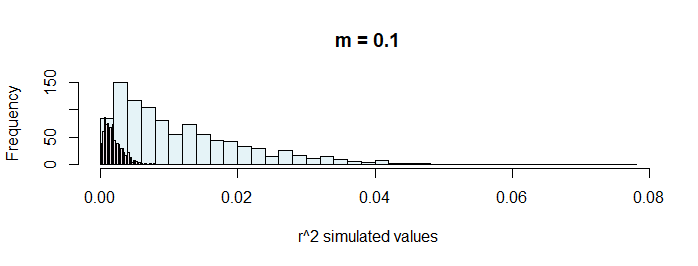
\includegraphics[scale=0.8]{8.png}%
    \caption*{Figure (8): The blue barchart shows the distribution for $l^2$  (for the 1000 synthetic datasets simulated) when the two populations have no migration (they are more dissimilar, hence higher $l^2$).
The black barchart is for the case when migration = 0.1.
In both scenarios the two populations have starting frequencies c(0.25,0.25,0.25,0.25).
Nevertheless, we still manage to pick up a clear signal on whether migration is happening or not.
}% 
\end{figure}%

\begin{figure}[H]
    
    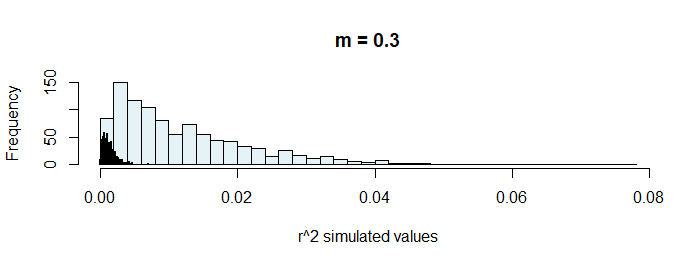
\includegraphics[scale=0.8]{9.png}%
    \caption*{Figure (9): Comparison with migration = 0.3, the difference is even clearer than in the former case 
}% 
\end{figure}%

I also carried out an identical analyisis but when population 2 is 10x bigger than population 1 ($N_e = 1,000$, $M_e = 10,000$).
In this case, due to limited computing power I only carried out 100 simulations, but the results were nevertheless good.

\begin{figure}[H]
    
    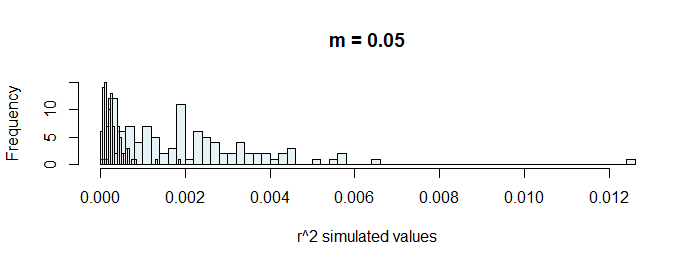
\includegraphics[scale=0.8]{10.png}%
    \caption*{Figure (10): Mainland-island scenario, comparison with migration = 0.05, good differentiability even with only 5\% migration
}% 
\end{figure}%
All the code is available at:\\
\url{
https://github.com/francescobarbara/UROP/tree/main/joint_r%5E2_measure/likelihood_ratio_test}

\section{Dissimilarity measure}
Given  2 genetic datasets (representing the 2 populations), we can easily calculate the between population $l^2$ and the two $r^2$  for many pairs of loci.
Suppose the recombination rates of these pairs are known (I work with 1000 pairs, because of limited computing power; more pairs $\implies$ better precision).

\begin{figure}[H]
    
    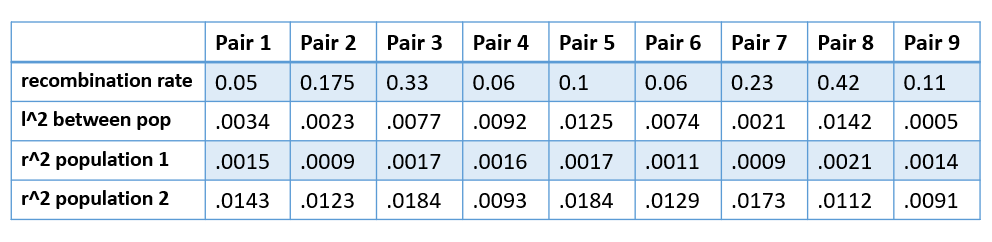
\includegraphics[scale=0.7]{11.png}%
    \caption*{Figure (11): Sample dataset
}% 
\end{figure}%

Suppose we have an estimate for the triplet $(N_{est}, M_{est}, migration_{est})$.
We want to see whether these estimates agree with the observed data.\\
Moreover, it can be seen in the figure below that when plotting $l^2$ values for two relatively high migration rates, the two empirical distributions differ, but not by much. We would ideally like to be able to differentiate these cases as well.

\begin{figure}[H]
    
    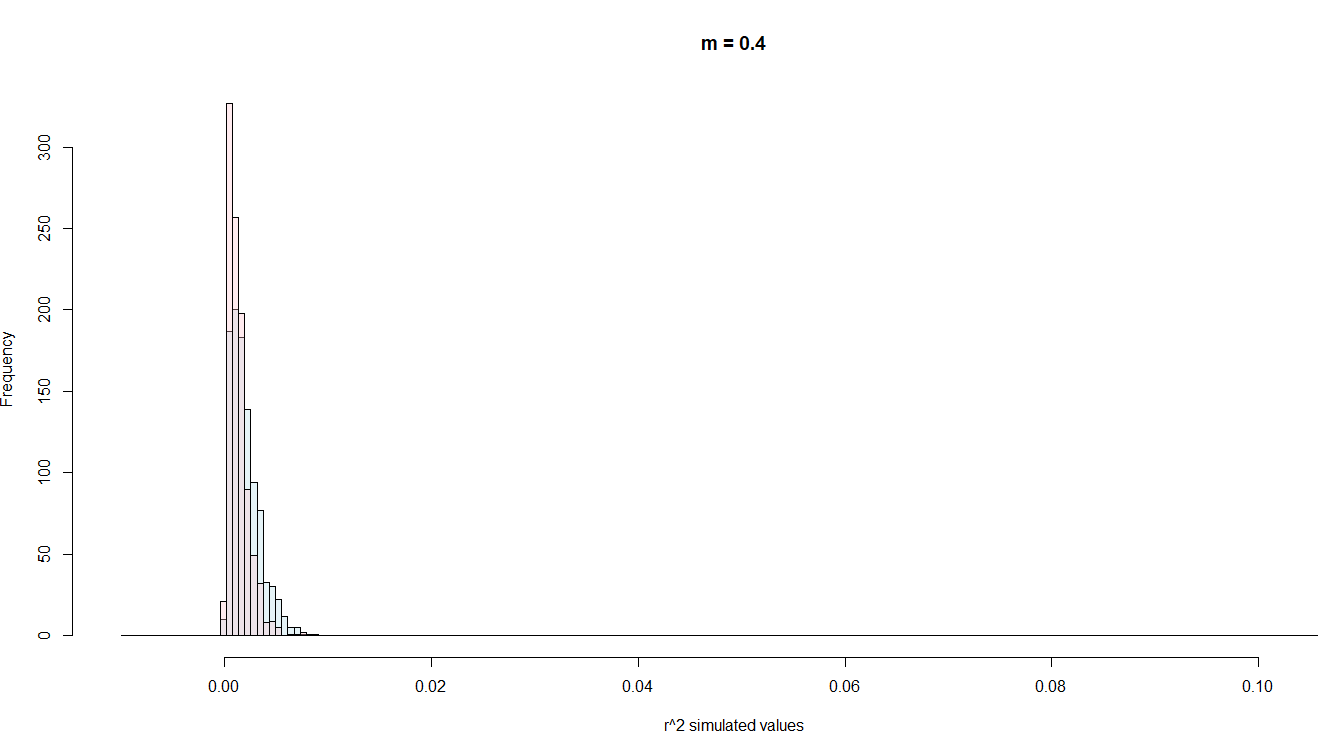
\includegraphics[scale=0.6]{12.png}%
    \caption*{Figure (12): Comparison between migration = 0.4 and migration = 0.1 
}% 
\end{figure}%

\noindent  For each pair / recombination rate:

\begin{figure}[H]
    
    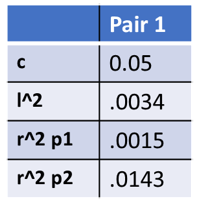
\includegraphics[scale=0.6]{13.png}%

\end{figure}%

\begin{enumerate}
  \item[1.] Simulate the 3 probability distributions of $l^2$ ,$ r^2_{pop1}$ , $r^2_{pop2}$ 
     under parameters $(N_{est}, M_{est}, migration_{est} , c)$. This is achieved by doing 100/1000 simulations (see later section for a deeper dive) of the C++ simulator under the given parameters. For each simulation, I take the frequencies at the last generation (generally generation 50 or 100, to give time to the smaller recombination rates to converge to equilibrium) and I calculate the values of $l^2$ ,$ r^2_{pop1}$ , $r^2_{pop2}$, this will be one data point used to construct the empirical cumulative distribution functions (ecdfs).

\end{enumerate}

\begin{figure}[H]
    
    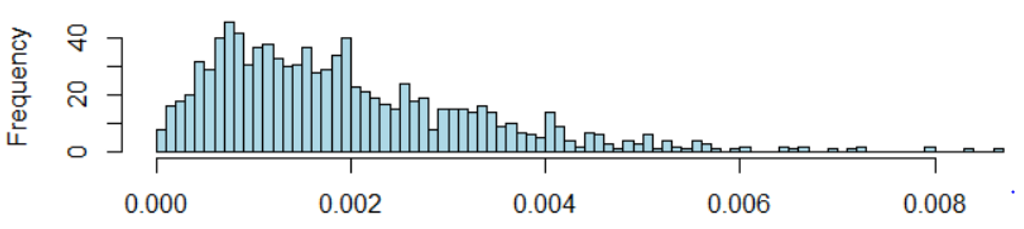
\includegraphics[scale=0.6]{14.png}%
    \caption*{Figure (14): Approximate distribution of  $r^2_{pop1}$ under parameters $(N_{est}, M_{est}, migration_{est} , c)$

}% 
\end{figure}%

\begin{enumerate}
  \item[2.] Compare the observed value of $r^2_{pop1}$ , (and do the same thing for $l^2$ , $r^2_{pop2}$)  with the simulated distribution.
Store the distance in terms of ‘cdf’ between the median of the simulated distribution and the observed value of $r^2_{pop1}$  (formally: the difference between 0.5 – i.e. the median -  and the empirical cumulative distribution evaluated at the observed $r^2_{pop1}$).
\end{enumerate}

\begin{figure}[H]    
    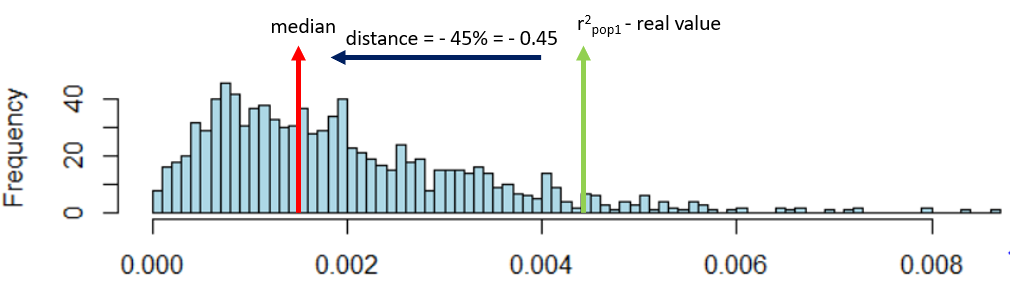
\includegraphics[scale=0.6]{15.png}%
\end{figure}%

\begin{enumerate}
  \item[3.] Sum together all the $3*n$ distances for the $n$ recombination rates, then take the a weighted average (I do a weighted average with 80\% weight to $l^2$ and 20\% to the $r^2$. A good way of thinking about these weights is the following: $r^2_{pop1}$ is sensible to $N_e$,  $r^2_{pop2}$ is sensible to $M_e$, while $l^2$ is sensible to all three $N_e$, $M_e$, $migr$; hence if we care `equally' about population estimates we should give a higher weight to $l^2$; I did many trials with different weights, and this choice seemed the most reasonable one)
\end{enumerate}

If $(N_{est}, M_{est}, migration_{est})$ are the real underlying parameters, the distances are 3*n uniform random variables between $[-0.5, 0.5]$, so their mean should be close to zero.

\subsection{Distribution of the dissimilarity mesure \textbf{$\rho$} under the null}
We want to be able to tell if the real data we observe could realistically come from two populations with parameters $(N_{est}, M_{est}, migration_{est})$. \\
\noindent Based on the previously defined dissimilarity measure, we developed the following statistical test.\\

\noindent $H_0$ : $(N_{est}, M_{est}, migration_{est})$ are the real parameters\\
\noindent Under $H_0$,  the $3*n$ distances shown earlier, are uniform random variables on [-0.5, 0.5]\\
\noindent We can exploit this:
$$\rho(N_{est}, M_{est}, migration_{est}) = abs( 1/n \cdot \sum_{k= 0}^{n} 0.8\cdot (U_{0k} - 0.5)
+ 0.1 \cdot (U_{1k} - 0.5) + 0.1 \cdot(U_{2k} - 0.5))$$
where $U_{ij}$ are i.i.d. $Unif[0,1]$\\

\noindent Remark: Suppose n = 1,000; then for ex. $U_{25,0}$ is independent with all the 2,997 $U_{ij}$ where $j \neq  25$ , but it will actually be correlated with $U_{25,1}$ and $U_{25,2}$. We approximate nevertheless with 3000 i.i.d. random variables.
$$ = abs( 0.8\cdot [1/n \cdot \sum_{k= 0}^{n} (U_{0k} - 0.5)]
+ 0.1 \cdot [1/n \cdot\sum_{k= 0}^{n} (U_{1k} - 0.5)] + 0.1 \cdot [1/n \cdot\sum_{k= 0}^{n} (U_{2k} - 0.5)] )$$ 
Since $U_{ik}$ and $U_{jk}$ with $i \neq j$ are independent:

$$ = abs( 0.8\cdot N(\mu = 0; \sigma^2 = \frac{1/12}{n}) + 0.1 \cdot N(\mu = 0; \sigma^2 = \frac{1/12}{n}) + 0.1 \cdot N(\mu = 0; \sigma^2 = \frac{1/12}{n}) )$$

Therefore the p-value for the test (that indicates how likely the real data is to come from the estimated parameters) can be defined as:\\
$$p-value = Prob(\rho_{theoretical} \ge \rho_{observed} | H_{0})$$
$$ = Prob(|\sqrt{\frac{0.66}{12 \cdot n}} N(0,1) | \ge \rho_{observed})$$
$$= Prob(N(0,1) \ge \sqrt{\frac{12 \cdot n}{0.66}}) + Prob(N(0,1) \le - \sqrt{\frac{12 \cdot n}{0.66}}) $$
$$= 2 \cdot(1- \Phi( \sqrt{\frac{12 \cdot n}{0.66}}))$$

\pagebreak

Let's see a couple of examples. Let $(N_{real}, M_{real}, migration_{real}) = (1000, 1000, 0.1)$ and $n = 100$.
The p-value for $(N_{est}, M_{est}, migration_{est}) = (1000, 1000, 0.1)$ is 0.39.
The p-value for $(N_{est}, M_{est}, migration_{est}) = (1000, 1000, 0.3)$ is 0.0028.\\

\noindent The above formulae work under the assumption that we know the three real cdfs for  $l^2$ , $r^2_{pop1}$ , $r^2_{pop2}$ (so we can map observed values back to [0,1] using the inverse of the cdf). However, we do not know the real cdf, we are approximating it with some empirical cdf (ecdf) created with simulated values (below n = 1000), under parameters $(N_{est}, M_{est}, migration_{est}, c)$.
$$ ecdf(real \: data; N_{est}, M_{est}, m_{est}) \approx Unif[0,1] \quad under \: H_0$$
\begin{figure}[H]    
    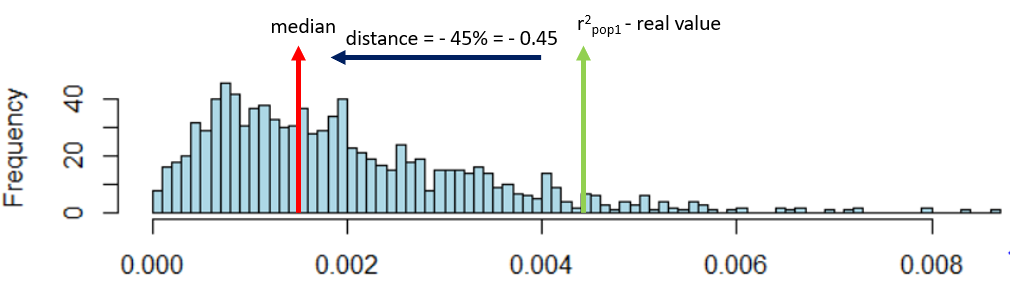
\includegraphics[scale=0.6]{15.png}%
\end{figure}%

How much extra variability does this introduce?\\

\noindent Rough explanation (hopefully helpful): Imagine you have $n = 1000$ loci, assume the 1000 recombination rates c are all different. Then you'll have to simulate 3000 different ecdfs under parameters $(N_{est}, M_{est}, migration_{est}, c)$.\\
\noindent Suppose these cdfs are quite rough (say you only use 100 points to build each ecdf). \\
\noindent You can imagine that for some c $ecdf(real \: data; N_{est}, M_{est}, m_{est},c)$ will be higher than it should be, while for others it will be smaller. For large number of pairs $n$ this should balance out.
\noindent However, for computational reasons (simulating 3000 different ecdfs for each triplets in the sequential Montecarlo was infeasible), I generally used 1000 recombination rates sampled from $\{0.05, 0.10, 0.15, ..., 0.45, 0.50\}$ so that I only had to simulate 20*3 cdfs. In this case the remark above of `errors cancelling out' does not hold anymore. For example suppose overall our 60 ecdfs are slightly shifted to the left, then the dissimilarity function will converge to a small positive value (we are subtracting 0.5 to the ecdf, in the picture we are actually doing the opposite, doesn't change anything). This value, however, will be much bigger than the expected standard deviation around zero which decreases by a factor of $\frac{1}{\sqrt{n}}$, (remember $|\sqrt{\frac{0.66}{12 \cdot n}} N(0,1)|$ is the distribution of our dissimilarity function under $H_0$. Therefore, even if $(N_{est}, M_{est}, migration_{est})$ is actually the correct estimate, we would get 0.00 p-values becuase our ecdfs are not precise enough.

\noindent We want to understand how many points for each ecdf we need, in order for the true distribtuion  $|\sqrt{\frac{0.66}{12 \cdot n}} N(0,1)|$ to emerge. For each of the following scenarios I calculated 100 values of $\rho(N_{real}, M_{real}, migration_{real})$ (dropped the absolute value, so I am dealing with a Gaussian) and compared this distribution to  $\sqrt{\frac{0.66}{12 \cdot n}} N(0,1)$  to check whether the mean and standard deviation are as expected.

\begin{figure}[H]
    
    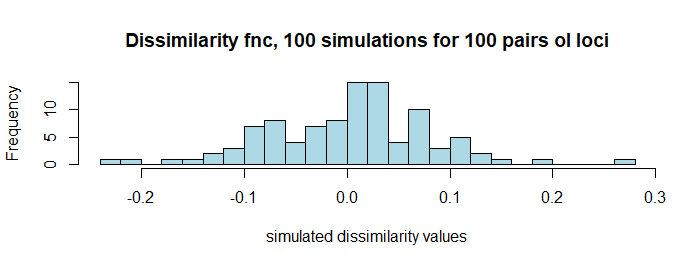
\includegraphics[scale=0.6]{16.png}%
    \caption*{Figure (16): number of points per ecdf = 100, pairs of loci n = 100; mean = 0.0014 (expected 0.00); standard deviation = 0.081 (expected 0.02)

}% 
\end{figure}%

\begin{figure}[H]
    
    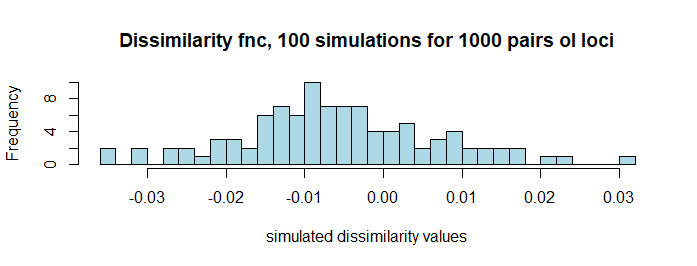
\includegraphics[scale=0.6]{17.png}%
    \caption*{Figure (17): number of points per ecdf = 100, pairs of loci n = 1000; mean = -0.005 (expected 0.00); standard deviation = 0.012 (expected 0.0074)

}% 
\end{figure}%

\begin{figure}[H]
    
    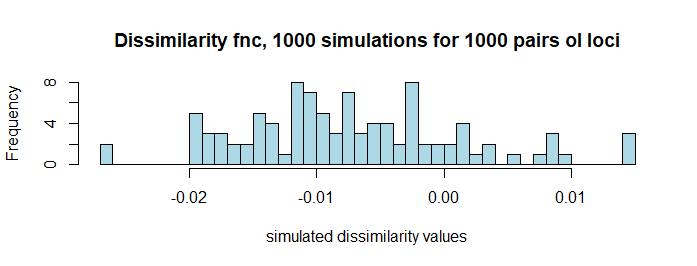
\includegraphics[scale=0.6]{18.png}%
    \caption*{Figure (18): number of points per ecdf = 1000, pairs of loci n = 1000; mean = -0.007 (expected 0.00); standard deviation = 0.0085 (expected 0.0074). The standard deviation is very close to the expected one, even with only 100 dissimilarity values simulated; very solid evidence in favour of the test developed

}% 
\end{figure}%

\subsection {Other possible dissimilarity measures}
In this section I briefly go through two possible adjustments of the above dissimilarity function.
\subsubsection {Austin's proposal}
I think Austin's comment was spot on. The rough idea is that, by summing all the $3n$ distances together if, for example $N_{est} >> N_{real}$ and $M_{est} << M_{real}$ then you'll have n terms of the sum $U_{1j} < 0$ and n terms $U_{2j} > 0$ and these will balance out giving a total sum close to zero.\\
\noindent It is not actually the case that these things balance out perfectly, and that there are triplets far from the true value such that 
 $\rho(N_{est}, M_{est}, migration_{est}) \le \rho (N_{real}, M_{real}, migration_{real})$ (the reason behind this is that $l^2$ is sensible to $N_e$, $M_e$ and $migr$ altogether). However, suppose $(N_{real}, M_{real}, migration_{real}) = (1000,1000,0.1)$, then it is true that $\phi(2000, 500, 0.1)$ is smaller than $\rho(2000,2000,0.1)$ even though these two estimated triplets are `equally bad'. This is not a desirable property but it can be easily fixed by taking three absolute values separately:
$$ |0.8\cdot [1/n \cdot \sum_{k= 0}^{n} (U_{0k} - 0.5)]|
+ |0.1 \cdot [1/n \cdot\sum_{k= 0}^{n} (U_{1k} - 0.5)]| + |0.1 \cdot [1/n \cdot\sum_{k= 0}^{n} (U_{2k} - 0.5)]|$$ 
$$ \approx 0.8\cdot |N(0, \frac{1/12}{n})| + 0.1 \cdot |N(0, \frac{1/12}{n})|+ 0.1 \cdot |N(0, \frac{1/12}{n})| \qquad under \: H_0$$

A similar test to that in section 6.1 can be devised (you can simulate very quickly 1 million triplets of Gaussians, and then see what the ratio of triplets that have values above the observed one; this will be the p-value that tells us how likely the observed data is to come from the estimated parameters).

\subsubsection {Euclidean distance, Beaumont(2010)}
My initial approach was, inspired by the Euclidean Distance Beaumont uses in its Sequential Montecarlo, was to sum the $3n$ normalized squared distances $(\frac{x_i - \mu}{\sigma})^2$. This gave much worse results than the `inverse cdf' approach. A nice and intuitive way to think about this is that, in this case, instead of using all the information contained in our 100/1000 simulated datapoints by creating an ecdf, we only keep track of two numbers (namely $\mu$ and $\sigma$). For example the two distributions below have same mean and variance, with the ecdf approach we would immediately be able to tell them apart, with Beaumont approach the results would be identical.

\begin{figure}[H]
    
    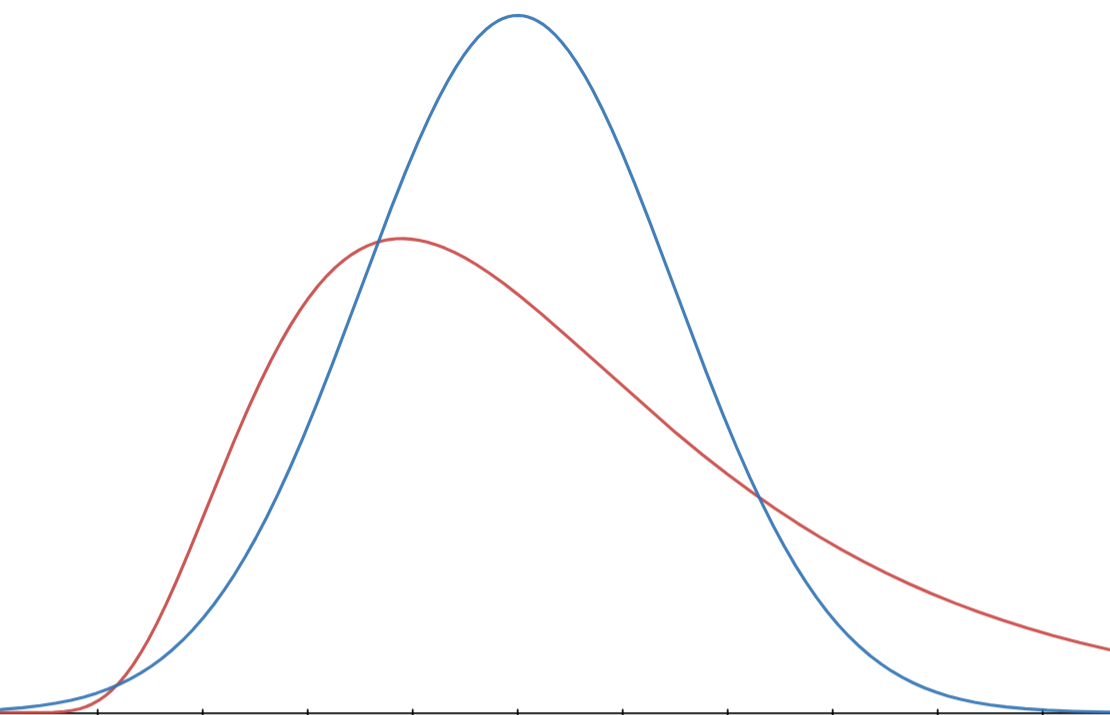
\includegraphics[scale=0.6]{19.png}%

\end{figure}%
All the code is available at:\\
\url{
https://github.com/francescobarbara/UROP/tree/main/approximate_bayesian_computation_ABC}

\section{Sequential Montecarlo}
\subsection{Algorithm outline}
\begin{enumerate}
  \item[$\bullet$] Hyper-parameters: \# layers/iterations (ideally around 10 ) ; \# triplets to simulate at each layer (30) ;  \# triplets to keep at each layer (5)
  \item[$\bullet$] Migration range is [0, 0.5]; Find an upper bound for $N_{real}$, $M_{real}$ by looking at $r^2_{pop1}$ , $r^2_{pop2}$  (remember migration will make your estimates biased upwards, but that’s ok as we just want an upperbound). Population ranges are $[0, N_{upp}]$ , $[0, M_{upp}]$.
  \item[$\bullet$] Sample 30 ‘triplets’ uniformly from this range, keep the 5 with lowest $\rho(N_{est}, M_{est}, migration_{est})$
  \item[$\bullet$] Sample the new layer (of size 30):
 \item[1.] Sample a ‘triplet’ from the previous layer ‘top 5’ , with probability proportional to $1/\rho(N_{est}, M_{est}, migration_{est})$   so good fits are sampled more often.
 \item[2.] Add Gaussian noise to the sampled triplet, with variance equal to the variance of the previous layer ‘5 best’ 
\item[$\bullet$] Pick the ‘top 5’ of the new layer; recurse until either you reach maximum \# layers or improvements stop

 \end{enumerate}
 
 \subsection{Comments on the algorithm}
 Techincal remark for Tin-Yu: if you want to implement some other variation of Sequential MC, have a look at \url{https://github.com/francescobarbara/UROP/tree/main/approximate_bayesian_computation_ABC}, the code is fully commented and highly modularized, so if you need to change some parts of the algorithm, you won't have to code the remaining 90\% of the algorithm.\\
 
 The algorithm was very expensive to run, especially if you wanted to have several layers. The convergence was not generally good enough (in the sense that if you created a 3d box containing all the triplets of the final layer, these would be too sparse to be a good -   i.e. narrow - confidence iterval)
 Below there are a few examples I run (using 6 layers).
 \begin{figure}[H]
    \centering
    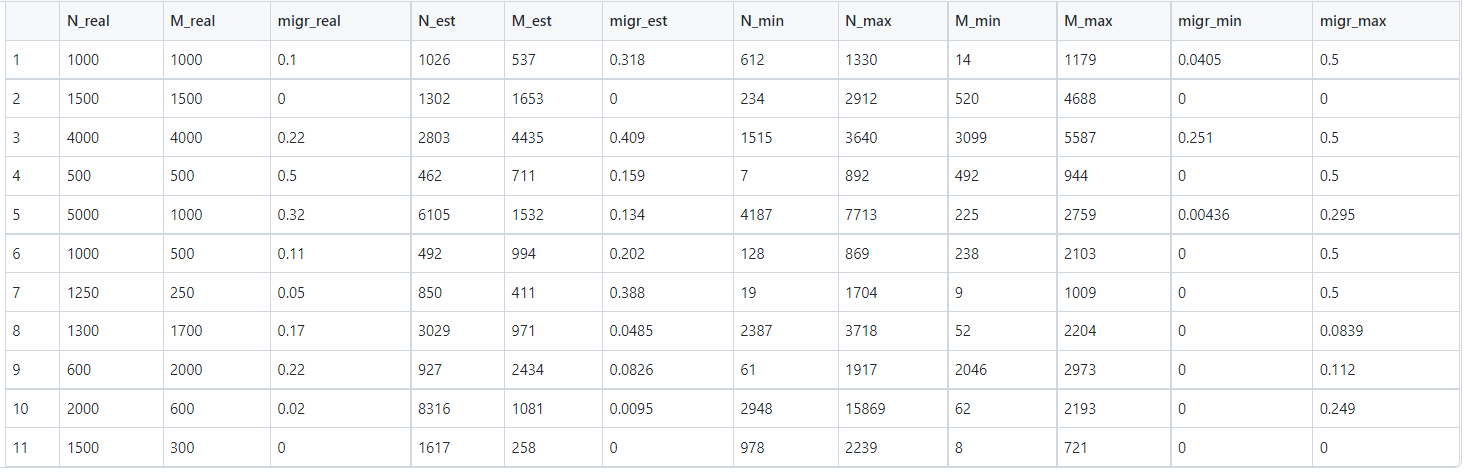
\includegraphics[scale=0.55]{20.png}%

\end{figure}%

\section{Final comments and what can be done next}

Between-population LD measure:  I think the idea was quite good. The only paper we found on this topic Sved (2010) (which uses identity-by-descent as a proxy for linkage disequilibrium) was not very convincing. Not much left to do here.\\

Dissimilarity measure: I saw `squared distances' being used a lot. Using the `cdf trick' gave much better results. Plus, using the cdf to map observations onto [0,1] is a common practice in statistics, so nothing too weird going on.\\
\noindent I think that, with the correction suggested by Austin (summing the 3 measures separately), this already looks quite good. \\
\noindent Still, some considerations could be made: \\
\noindent 1. Insted of summing the three absolute values of the averages, we could do something else (for example, it you take the sum of the 3 squares, with weights 1,1,1, then you have a $\chi^2_3$ )\\
\noindent 2. The weights 0.8, 0.1, 0.1 I used were based on the empirical performance of the sequential MC (which needs to be changed) so these could be modified\\

Sequential MC: Right now it's pretty bad (Beaumont's algorithm performs even worse). One thought I have had in mind is the following: \\
\noindent If we plot the values of the dissimilarity function over the the 3d space of $(N_e, M_e, migr)$ we can expect this function to be convex with a minimum at the real values $(N,M,migr)$ (imagine a parabola in 4d). Then for each data point we could try to figure out the `gradient' at the point (essentially in which diretion the minimum is) by simulating some extra points around the previous data point.\\
\noindent More radical changes (moving away from the sequential MC framework) could also be a solution.
\end{document}\\